\graphicspath{ {figures/conclusion/} }

%%%%%%%%%%%%%%%%%%%%%%%%%%%%%%%%%%%

\chapter{Conclusions}
\label{ch:conclusion}

The preceding chapters are unified by their pursuit of a common question: how do the structure and function of gene regulatory networks control cell fate decisions and yield emergent properties at the organismal scale? Each chapter combined quantitative data and mathematical analysis to address subtle aspects of this question in a unique way. The following sections provide an introspective summary of how each chapters findings, and the lessons learned therein, impact the present understanding and future research directions of quantitative, developmental, and systems biology. 

\section{Implications for developmental and systems biology}

Chapter \ref{ch:clones} introduced a computational framework for automated analysis of genetic mosaics; a class of experiments commonly used to probe cell fate decisions \textit{in situ} \cite{Germani2018,Atkins2019}. The framework combines computer vision and statistics to automate the labor-intensive steps of a quantitative work-flow, enabling automated and systematic comparison of cells subject to control and perturbation conditions in an otherwise equivalent background.

Quantitative mosaic analysis is not new, nor is it uncommon in high profile publications \cite{Dai2017,Gavish2016,Li2018}. Yet, these studies deploy an irreproducible mix of ad hoc implementations and costly commercial software. Worse still, qualitative analysis pervades less prominent corners of the literature. Contributing a fully automated framework to the open-source ecosystem will make quantitative mosaic analysis equally accessible to the entire community. A unified framework will also dramatically simplify the reproduction of existing analyses. Chapter \ref{ch:clones} therefore advances the quantification of developmental biology by adding potential for rigor and reproducibility where they are currently lacking.

Chapter \ref{ch:ratio} explored a novel cell fate decision mechanism underlying photoreceptor specification in the \textit{Drosophila} larval eye. Computer vision techniques were used to extract quantitative measurements of Pnt and Yan dynamics from a wealth of confocal microscopy data. Statistical analysis revealed that differentiation is driven by dynamic changes in the ratio between Pnt and Yan, and is agnostic to changes in their absolute concentrations as long as the ratio remains constant. The data therefore provide the first direct evidence that cell fate decisions can be triggered by changes in the relative abundance of separate transcription factors. This finding rebukes the canonical model of photoreceptor specification \cite{Graham2010}. More importantly, it adds a new dimension to our understanding of how multiple transcription factors cooperatively control cell fate decisions, with broad implications for many developmental contexts within and beyond \textit{Drosophila}. 

The ratiometric sensing mechanism identified in Chapter \ref{ch:ratio} adds to a growing body of evidence that cells are able to sense relative changes in the abundance of GRN components \cite{Goentoro2009a,Frick2017}. These discoveries are exciting because relative sensing could potentially isolate cell fate decisions from environmental sources of variation. This is because environmental fluctuations would likely manifest as correlated extrinsic noise that affects all GRN components in a similar manner, causing absolute but not relative concentrations to vary between cells. Relative sensing might then increase fitness in variable environments. 

Regulatory interactions may provide additional layers of stability. Dual-reporter experiments have shown that regulation buffers cell-by-cell differences in yeast gene expression to enhance the precision of decisions to commit to a mating response phenotype \cite{Colman-Lerner2005}. Indeed, Chapter \ref{ch:metabolism} also showed that the microRNA miR-7 buffers Yan expression levels, and by extension R cell fate decisions, against varying biosynthesis capacity. Perhaps future experiments could address how Pnt levels are affected before and after IPC ablation in $yan^{\Delta miR\hyphy 7}$ mutants. 

These observations reflect a central theme of this dissertation; the structure and function of developmental GRNs dictate the robustness of cell fate decisions to environmental variation. Chapter \ref{ch:metabolism} directly embraced this sentiment. It proposed a new theory to explain why the regulatory networks that coordinate cell fate decisions often contain many seemingly redundant repressors acting upon the same target genes. The theory posits that auxiliary negative regulators mitigate erroneous cell fate decisions when cells are rapidly metabolizing, and implies that auxiliary repressors may help GRNs adapt their behavior to environmentally driven variation in cell metabolism. The theory is supported by a diverse collection of experiments in which repressor loss-of-function phenotypes were reversed when biosynthesis rates were slowed. A quantitative modeling framework was used to explore the mechanistic origin of this effect, and theoretically demonstrated that auxiliary repressors could avert erroneous decisions by expanding cells capacity to buffer excess protein expression. Quantitative measurements of transcription factor activity confirmed the hypothesized mechanism in vivo.

Chapter \ref{ch:intro} introduced the idea that developmental GRNs guide organisms through a tortuous journey from embryo to adulthood. The journey is not a sprint. Rather, cells must carefully navigate the many twists and turns of developmental programs; rapidly synthesizing GRN components when and where they are needed, then degrading them with equal urgency. Protein synthesis and degradation machineries supply the engine and brakes needed to negotiate these obstacles (Fig. \ref{fig:conc:fig0}A). Individuals stand to benefit from completing the journey quickly because they are generally vulnerable until adulthood, with little means to defend themselves against predation and other dangers. They could naively swap out the engine for something more potent, but adding power escalates risk, particularly around sharp corners (Fig. \ref{fig:conc:fig0}B). Simultaneously upgrading the brakes is a winning strategy (Fig. \ref{fig:conc:fig0}C). Analogously, evolution could accelerate development by expanding biosynthesis capacity. The resultant boost in protein expression would strain each cell's ability to localize distinct GRN activities in time, causing increased risk of erroneous fate decisions that lead to the emergence of deleterious phenotypes. However, by selecting for auxiliary repressors, cells could tolerate faster biosynthesis rates without compromising the quality of fate decisions. The data presented in Chapter \ref{ch:metabolism} confirm this hypothesis by illustrating the inverse perspective. Repressors were shown to be dispensable when metabolism was slow, much in the way that brakes aren't needed to round corners at low speed.

\begin{figure}[h!]
\centering
\includegraphics[scale=1.0]{./figure_0A}
\caption[The race from embryo to adulthood.]{\textbf{The race from embryo to adulthood.} Individuals must navigate the many twists and turns of the developmental program to reach the finish line. (A) Slow and steady loses the race. (B) Adding power improves acceleration, but increases the risk of failure. (C) Adding power along with better brakes is a winning strategy. The analogous experimental conditions are (A) slow metabolism without auxiliary repression, (B) fast metabolism without auxiliary repression, and (C) fast metabolism with auxiliary repression. This configuration is equivalent to wildtype, suggesting it consistently wins the race.}
\label{fig:conc:fig0}
\end{figure}

This line of reasoning implies that a novel evolutionary driving force may shape the structure and function of developmental gene regulatory networks. Shorter generational times confer a selective advantage beyond reducing individuals exposure during infancy. They facilitate rapid exploration of the phenotypic landscape, enabling fast adaptation to variable environments. GRNs should therefore be expected to incorporate any topological features that allow development to proceed more quickly. The abundance of seemingly redundant regulation found in developmental GRNs certainly appears to support this hypothesis, and thus reinforce our contemporary understanding that robustness is a fundamental organizational principle underlying the evolution of biological systems \cite{Kitano2004,Stelling2004}. 

The findings also contribute to an emerging view that cells capacity to rapidly adjust protein homeostasis directly affects organismal fitness and health \cite{Visscher2016,Tollerson2018,Burnaevskiy2018}. The assertion is backed by convincing experimental evidence. Burnaevskiy et al. used a dual-reporter scheme in \textit{C. elegans} to show that cellular differences in the abundance of protein synthesis machinery manifest in the population-wide penetrance of adult phenotypes. The authors went on to speculate that longevity might be similarly be affected \cite{Burnaevskiy2018}. Tollerson et al. showed that Elongation factor P alleviates a translational bottleneck caused by ribosomal queuing in \textit{E. coli}, facilitating adaption to environmentally-driven increases in cell metabolism \cite{Tollerson2018}. Chapter \ref{ch:metabolism} contributes unique evidence that the accuracy of cell fate decisions depends upon cells ability to dynamically balance the push and pull of protein synthesis and degradation. 

% ================================================ FUTURE DIRECTIONS
\section{Avenues for further exploration}

This dissertation prompts several exciting new directions for future research. This section begins with a survey of those that merit further attention, before elaborating on some preliminary analyses to guide prospective efforts.

Chapter \ref{ch:ratio} proposed that R cell fate commitment in the larval eye is driven by dynamic changes in the relative abundance of Pnt and Yan. Experimental evidence was limited to correlative observations because intrinsic regulation precluded direct manipulation of the Pnt-to-Yan ratio by varying gene dosage. Future studies could rigorously confirm the hypothesis by applying the same gene dosage perturbations in a genetic background that lacks the complete set of regulatory interactions needed to stabilize the Pnt-to-Yan ratio. Disrupting the ratio control mechanism would first require characterizing its biomolecular implementation. Computational simulations could explore the space of plausible GRN topologies, then leverage insight derived from existing experimental data to distill a manageable number of options for experimental validation. Establishing an unambiguous picture of R cell fate commitment might then allow for a complete model of retinal patterning dynamics, as is an ongoing mission among computational biologists \cite{Lubensky2011,Gavish2016}.

Chapter \ref{ch:ratio} used an equilibrium modeling framework to explore the effect of \textit{cis}-regulatory interactions between Yan monomers on the equilibrium binding occupancy of promoters regulated by Pnt and Yan. The approach was inspired by the work of Hope et al., who used an equivalent model, limited to a single binding component, to explore how the \textit{cis}-regulatory syntax of target genes modulates transcriptional output \cite{Hope2017}. The multi-species implementation introduced in Chapter \ref{ch:ratio} was comparatively underutilized. Future studies could ask many questions related to how \textit{cis}-regulatory syntax modulates the transcriptional output of genes regulated by two or more polymerizing transcription factors. How do the number and arrangement of individual binding sites modulate transcriptional output? What about the spacing or distribution of high and low affinity sites? What if anti-cooperative or steric interactions are included? Does the number of unique binding species matter? All of these questions could readily be explored using the open-source platform developed to support this dissertation (see Appendix \ref{appendix:software}).

The theory developed in Chapter \ref{ch:metabolism} posits that auxiliary repressors stabilize cell fate decisions against environmental variation in cells capacity to synthesize and degrade proteins. This assertion was backed by both experiments and computational analysis showing that repressors were dispensable when either ATP turnover or translation capacity were reduced. It is well known that many mutant phenotypes are also suppressed in animals raised at low temperatures. Future studies could ask whether reduced temperature imparts similar effects on the GRN dynamics that govern cell fate decisions. From a modeling perspective, the primary challenge would be deciding precisely how to incorporate the relative effects of temperature on the protein synthesis and degradation machineries. The analogous decisions were comparatively obvious for \textit{ILP2-GAL4 UAS-Rpr} and \textit{RP} mutants, in which protein synthesis is disproportionately affected. In principle, experimental efforts to quantify the dependence of protein synthesis and degradation rates on temperature could prove fruitful.

Alternatively, researchers could computationally survey the landscape of plausible relationships between proteostasis and the environment to identify conditions under which auxiliary repressors are dispensable. For instance, consider the simplest possible model of protein expression dynamics (Fig. \ref{fig:conc:fig1}A):
\begin{equation}
\label{eq:simple_base}
\frac{dP}{dt} = kI - \gamma P
\end{equation}
where $P$ and $I$ are the protein and stimulus levels, and $k$ and $\gamma$ are the synthesis and degradation rate parameters. Repressors may be implemented as proportional feedback, as they were in Chapter \ref{ch:metabolism}:
\begin{equation}
\label{eq:simple_repressor}
\frac{dP}{dt} = kI - \gamma P - \eta P
\end{equation}
where $\eta$ is the feedback strength. The frequency of developmental errors induced by losing the repressor is readily evaluated using the same procedure described in Chapter \ref{ch:metabolism} (Fig. \ref{fig:conc:fig1}B). Rather than hard-coding an explicit dependence of $k$, $\gamma$, and $\eta$ on environmental conditions, each parameter can be scaled by a latent dimension $\lambda$ that reflects the environmental state of the cell:
\begin{equation}
\begin{aligned}
k &\propto \lambda^{\nu_k}  \\
\gamma &\propto \lambda^{\nu_{\gamma}}  \\
\eta &\propto \lambda^{\nu_{\eta}}
\end{aligned}
\label{eq:parameter_dependence}
\end{equation}
where $\nu_k$, $\nu_{\gamma}$, and $\nu_{\eta}$ define the respective sensitivities of synthesis, degradation, and feedback strength to environmental conditions. Consider an example in which the environmental state of the cell is halved relative to some reference condition, i.e. $\lambda = \lambda_{0} / 2$. For $\nu_{i \in {k,\gamma,\eta}} = 1$, parameter $i$ is also halved. If $0 < \nu_i < 1$ or $\nu_i > 1$, parameter $i$ exhibits sub- or super-linear dependence on the environment, respectively. Finally, $\nu_i < 0$ implies that parameter $i$ should actually increase when $\lambda$ is halved. 

The robustness checks presented in Section \ref{metabolism:robust} surveyed a handful of discrete values for the model parameters analogous to $\nu_k$, $\nu_{\gamma}$, and $\nu_{\eta}$. The scaling assumptions used to represent conditions of reduced energy metabolism throughout Chapter \ref{ch:metabolism} were loosely equivalent to $(\nu_k, \nu_{\gamma},\nu_{\eta}) = (1,0,2)$. Applying the same assumptions to the simplified model recapitulates a core result of Chapter \ref{ch:metabolism}; error frequency is dependent upon the environmental state of the cell (Fig. \ref{fig:conc:fig1}C,D).

\begin{figure}[h!]
\centering
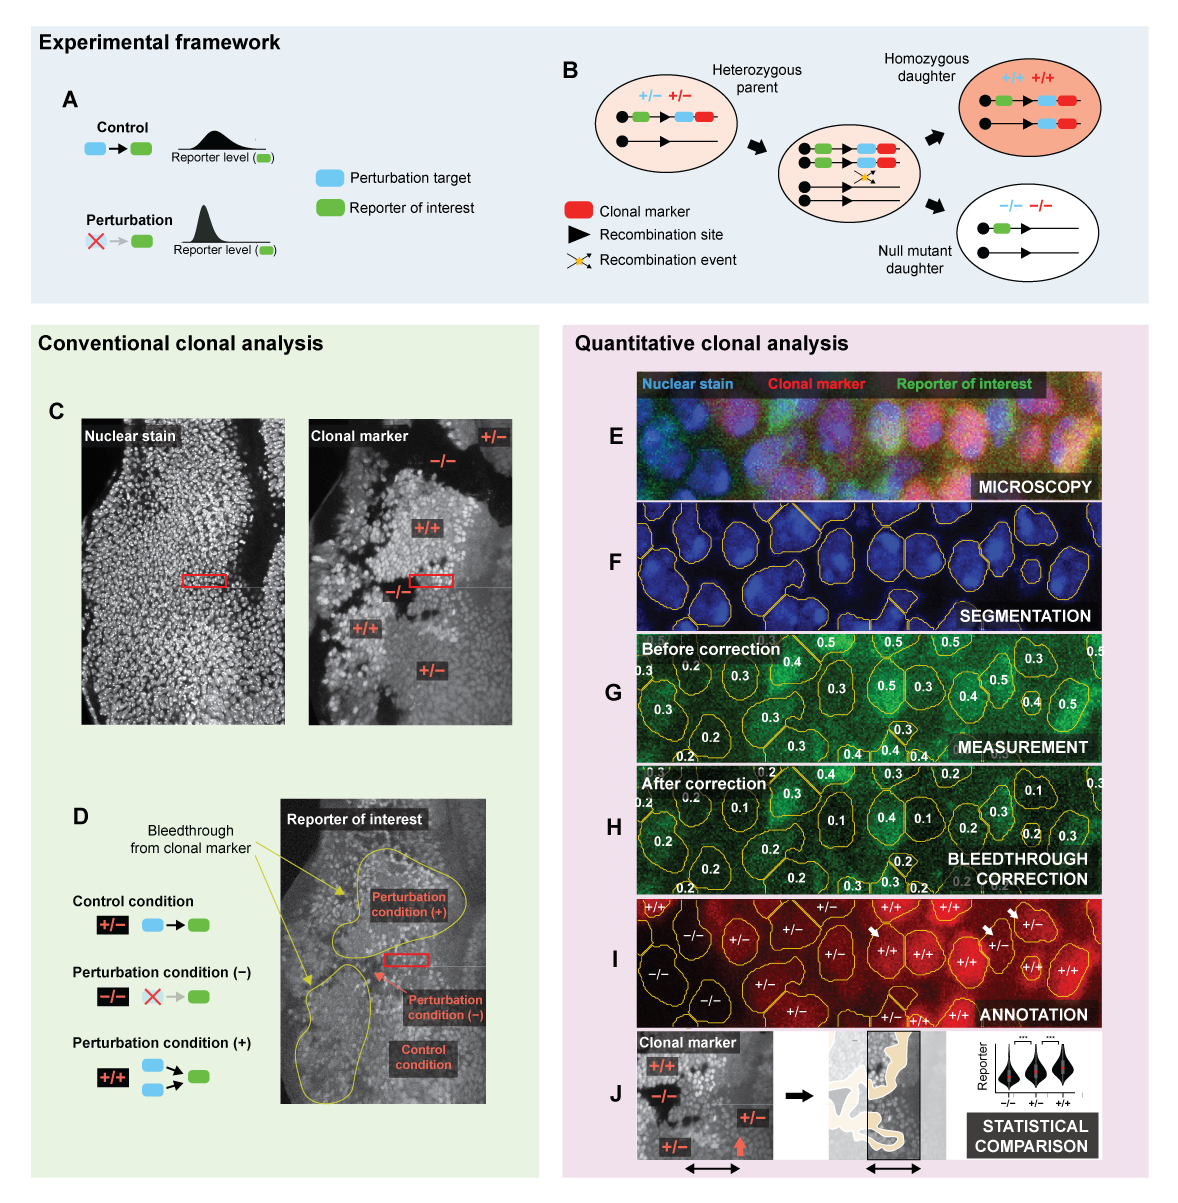
\includegraphics[scale=1.0]{./figure_1}
\caption[Simplified framework for modeling the loss of an auxiliary repressor.]{\textbf{Simplified framework for modeling the loss of an auxiliary repressor.} (A) Schematic representation of protein expression in response to a transient input. Output is subject to regulation by a single auxiliary repressor. (B) Simulated emergence of developmental errors. Simulations may be performed with (purple) or without (grey) the auxiliary repressor. Lines reflect a random sample of 5000 trajectories. The two sets of trajectories are compared when 99\% of trajectories simulated with the repressor cross a threshold value (dashed line). Without the auxiliary repressor, very few trajectories successfully cross the threshold. (C) Graphic representation of the relation between environmental conditions and the rate parameters that dictate protein synthesis, degradation, and repressor strength. (D) Error frequency is dramatically suppressed by a change in environmental conditions. }
\label{fig:conc:fig1}
\end{figure}

Combined, equations \ref{eq:simple_repressor} and \ref{eq:parameter_dependence} facilitate continuous enumeration of the phase diagram spanned by $\nu_k$, $\nu_{\gamma}$, and $\nu_{\eta}$ in order to identify the range of scaling assumptions under which auxiliary repressors may be dispensable. Performing this exercise revealed that induced error frequencies are highest when the strength of the removed repressor is more sensitive to the environment than the intrinsic rate of protein turnover (Fig. \ref{fig:conc:fig2}A, region IV). The same is true of error frequency suppression, indicating that highly sensitive repressors have the highest propensity to become dispensable (Fig. \ref{fig:conc:fig2}B, region IV). This observation is consistent with intuition, as environmental conditions that limit the influence of a repressor would also be expected to mitigate the impact of its removal. 

This preliminary analysis could guide the design of future experiments that survey the effects of temperature on mutations that compromise repressor function. For example, experiments could quantify $\nu_k$, $\nu_{\gamma}$, and $\nu_{\eta}$ for a particular cell-fate determinant by measuring steady-state protein levels in both wildtype and repressor loss-of-function mutants across a range of temperatures. They could then use the model to generate testable predictions for alternate temperatures.

\begin{figure}[h!]
\centering
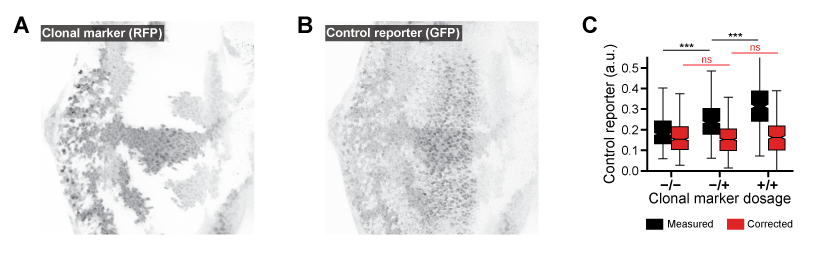
\includegraphics[scale=1.0]{./figure_2}
\caption[Suppression depends on parameter sensitivity to the environment.]{\textbf{Suppression depends on parameter sensitivity to the environment.} Phase diagrams span a range of protein degradation and repressor strength sensitivities to environmental conditions. Heatmaps show (A) error frequency induced by the loss of an auxiliary repressor when $\lambda = \lambda_0$ and (B) change in error frequency when $\lambda = \lambda_0 / 2$. All simulations use $k = 1$, $\gamma = 0.001$, $\eta = 0.001$, and $\lambda_0 = 1$. Dark blue indicates strong error frequency suppression. Red numerals label quadrants. The example shown in Fig. \ref{fig:conc:fig1} is taken from quadrant IV. }
\label{fig:conc:fig2}
\end{figure} 

Chapter \ref{ch:metabolism} also raises the question of whether any other features of GRNs are dispensable under certain environmental conditions. For instance, how about promoters? Preliminary analysis may again provide some insight to guide future work. Consider another scenario in which an auxiliary promoter is added to the simple model given by Equation \ref{eq:simple_base}:
\begin{equation}
\label{eq:simple_promoter}
\frac{dP}{dt} = kI + k_{aux}I - \gamma P
\end{equation}
where $k_{aux}$ is the rate constant for synthesis driven by the auxiliary promoter. The relative influence of the auxiliary promoter is given by its strength relative to the primary promoter, i.e. $log_2 ( k_{aux} / k )$. The respective sensitivities of both promoters and degradation to environmental conditions are again parameterized in terms of $\lambda$:
\begin{equation}
\begin{aligned}
k &\propto \lambda^{\nu_k} \\
k_{aux} &\propto \lambda^{\nu_{k-aux}} \\
\gamma &\propto \lambda^{\nu_{\gamma}} \\
\end{aligned}
\end{equation}
The simulation procedure described in \ref{ch:metabolism} is readily modified to evaluate the frequency of developmental errors induced by removing the auxiliary promoter, i.e. by setting $k_{aux}=0$. Intuition suggests promoter loss should cause a decrease in output protein levels. Error frequency is therefore redefined to reflect the extent to which protein is \emph{under-expressed} when the auxiliary promoter is removed. The metric is evaluated by computing the fraction of trajectories simulated with a single promoter that fail to reach the lower bound of trajectories simulated with both promoters. Surveying a range of promoter strengths and relative influences reveals that error frequencies are most severe when strong and influential auxiliary promoters are removed (Fig. \ref{fig:conc:fig3}A). Figure \ref{fig:conc:fig3}B shows the subsequent change in error frequencies when $(\nu_k, \nu_{k-aux},\nu_{\gamma}) = (1,1,1)$ and $\lambda = \lambda_0 / 2$. The phase diagram is punctuated by a diagonal band in which error frequencies are suppressed. Below this band, suppression is minimal because the auxiliary promoter is inconsequential to normal protein expression dynamics (Fig. \ref{fig:conc:fig3}A,B, region I). Above it, removing the auxiliary promoter imparts a severe perturbation that cannot be recovered by the proposed change in environmental conditions (Fig. \ref{fig:conc:fig3}A,B, region II). Similar zones arise when the equivalent procedure is performed using the model of auxiliary repressor loss defined by equation \ref{eq:simple_repressor} (Fig. \ref{fig:conc:fig4}). Here, the influence of the auxiliary repressor is defined relative to the intrinsic degradation rate, i.e. $log_2 ( \eta / \gamma )$. 

\begin{figure}[h!]
\centering
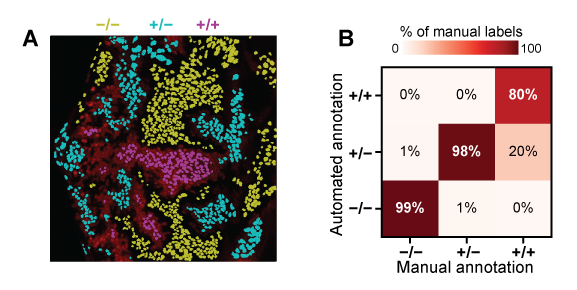
\includegraphics[scale=1.0]{./figure_3}
\caption[Phase diagram of auxiliary promoter loss.]{\textbf{Phase diagram of auxiliary promoter loss.} 
Phase diagrams span a range of auxiliary promoter strengths and influences. Heatmaps show (A) error frequency induced by the loss of the auxiliary promoter when $\lambda = \lambda_0$ and (B) change in error frequency when $\lambda = \lambda_0 / 2$. All simulations use $\gamma = 0.001$ and $\lambda_0 = 1$. Dark blue indicates strong error frequency suppression. Perturbations targeting promoters in region I are inconsequential. Those targeting promoters in region II are too severe to be recovered. Blue band is the Goldilocks zone.}
\label{fig:conc:fig3}
\end{figure}

\begin{figure}[h!]
\centering
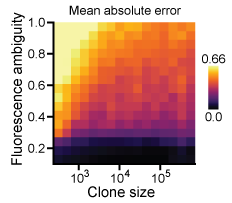
\includegraphics[scale=1.0]{./figure_4}
\caption[Phase diagram of auxiliary repressor loss.]{\textbf{Phase diagram of auxiliary repressor loss.} 
Phase diagrams span a range of auxiliary repressor strengths and influences. Heatmaps show (A) error frequency induced by the loss of the auxiliary repressor when $\lambda = \lambda_0$ and (B) change in error frequency when $\lambda = \lambda_0 / 2$. All simulations use $k = 1$ and $\lambda_0 = 1$. Dark blue indicates strong error frequency suppression. Perturbations targeting repressors in region I are inconsequential. Those targeting repressors in region II are too severe to be recovered. Blue band is the Goldilocks zone.}
\label{fig:conc:fig4}
\end{figure}

The bands observed in Figures \ref{fig:conc:fig3}B and \ref{fig:conc:fig4}B indicate the existence of a Goldilocks zone in which perturbations are strong enough to be felt but weak enough to be recoverable. In other words, there exists a finite and continuous range of conditions in which error frequencies can be suppressed by slowing biosynthesis. Given appropriate knowledge of promoter and repressor strengths, a model could inform the selection of experimental perturbation targets that fall within the range. Such an approach would also require quantification of $\nu_i$ and $\lambda$ for a given model system.

The value of the models defined by equations \ref{eq:simple_repressor} and \ref{eq:simple_promoter} lies in their simplicity. Because each strictly employs linear kinetics, the stochastic dynamics are analytically tractable via a closed system of moment equations \cite{Sotiropoulos2011}. Even the more complex models presented in Chapter \ref{ch:metabolism} are approximately solvable, courtesy of modern moment closure and finite state projection techniques \cite{Singh2011,Munsky2006}. Future theoretical efforts could be directed toward the development of a complete analytical framework for studying the interplay of GRN dynamics, cell fate decisions, and the environment. An analytical platform would vastly reduce the computational burden imposed by the numerical methods used to conduct all of the analysis presented in this section and throughout Chapter \ref{ch:metabolism}. It would also expedite fitting the model to experimental data in order to generate testable predictions. 

% ================================================ PERSPECTIVES ON QUANT BIO
\section{Perspectives for quantitative biology}

This dissertation surveyed developmental cell fate decisions through a quantitative lens. It used numbers and equations to derive nuanced understanding of processes that are notoriously difficult to characterize. In many cases, doing so required forcible reconciliation with time-honored traditions in biological analysis. Two major obstacles encountered along the way merit further discussion.

First, models should fit the data; not the other way around. While it may be possible to coax data into a conventional framework, tailoring one appropriate for the task at hand will generally return more meaningful insight. Mathematical flexibility was a key strength of this dissertation. Each chapter leveraged a customized modeling framework to elicit deeper meaning out of experimental data than would have been possible using conventional techniques. 

Chapter \ref{ch:clones} deployed a Bayesian statistical framework to infer cell genotypes from an image of clonal marker expression. Biological intuition suggests it should have enforced detection of three distinct components strictly delimited by clonal marker level. Instead, the model was designed to tolerate an arbitrary number of components that also considered spatial context, which were later aggregated into the three anticipated genotypes. This empirical formulation buffered uncertainties imparted by expression heterogeneity and imaging noise to improve annotation performance overall.

Chapter \ref{ch:ratio} used an equilibrium binding model to explore how \textit{cis}-regulatory interactions between Yan monomers bias the transcriptional output of genes simultaneously regulated by Pnt. Conventional wisdom suggests a competitive binding model using the Hill-Langmuir equation would be appropriate \cite{Gesztelyi2012}. Instead, a statistical mechanical approach was adapted from earlier work by Hope et al. \cite{Hope2017}. Contrary to the empirical strategies used in other chapters, this model substantially \emph{increased} the resolution of analysis. Doing so provided detailed mechanistic insight into the intricacies of polymerizing transcription factors, which would have otherwise been inaccessible (see Fig. \ref{fig:ratio:figS5}C). 

Chapter \ref{ch:metabolism} sought to model the dynamic output of GRNs controlling a broad spectrum of cell fate decisions. The conventional first step would have been to identify and consolidate all known regulatory interactions in each system. Such an endeavor was certainly possible for Yan-mediated control of retinal patterning, as the pertinent interactions have been studied for decades \cite{Ready1976a,Rebay1995,Rohrbaugh2002,Li2009b,BoisclairLachance2014} and in some cases quantified \cite{Pelaez2015a}. Chapter \ref{ch:metabolism} instead drew inspiration from control theory to develop a model strictly concerned with the two salient features of pulsatile dynamics; the magnitude of induction and timescale of decay. The model jettisoned the molecular details of protein expression and regulation in each system, instead favoring a coarse-grained depiction of output dynamics. The reductionist approach was vital to simultaneously depicting the behavior of a diverse assortment of cell fate decisions.

Chapter \ref{ch:metabolism} was also forced to circumvent the second major obstacle: The resolution of analysis should match the resolution of the data. Biological networks are complex, often far more complex than we can intuitively comprehend. Their emergent behavior arises from the collective interactions of numerous components, many of which are often unknown. These uncertainties make it particularly dangerous to think of a GRN as the sum of its parts. Similarly, predictions are all but meaningless when made by aggregating disparate interactions that were characterized in isolation.

Despite slowly coming under scrutiny, these practices remain tragically common. They are perhaps most strongly embodied in the abundance of cartoons that purport to depict systems level-behavior with a compendium of qualitative regulatory interactions. Figure \ref{fig:ratio:fig7}A provides a modest example. This cartoon is harmless in isolation, but problems arise when unsuspecting viewers ascribe physical meaning to the various interactions. After all, there is no unified standard to define what an arrow, or ``edge,'' means. A single edge might actually represent an entire sub-network of complex nonlinear processes. Intermediate steps within an edge might even interact with other intermediates in other edges drawn elsewhere in the diagram. Cartoons are thus rife with ambiguity that hinders the communication of otherwise outstanding research. For instance, a basic attempt to simulate the system shown in Figure \ref{fig:ratio:fig7}A will reveal that the illustrated ``regulatory loop'' cannot maintain a constant Pnt-to-Yan ratio in response to varying \textit{pnt} or \textit{yan} gene dosage (data not shown). Yet, Figure \ref{fig:ratio:fig7}A was necessary because these depictions are so deeply ingrained in the biological literature that the representation in Figure \ref{fig:ratio:fig7}B would likely be misconstrued without it.

This ambiguity starkly contrasts the standardized descriptive languages commonly used in engineering \cite{Lazebnik2004}. To be fair, most human-engineered systems do not suffer the same extent of uncertainty as their biological counterparts. Notable exceptions arise in electrical, chemical, and biomolecular engineering. Autonomous vehicles, advanced robotics, process plants, and synthetic biological circuits must all contend with disturbances whose origin and character may be unpredictable or unknown. Fortunately, a viable solution to this challenge already exists. Control theory emphasizes an empirical representation of systems-level dynamics that is easily matched to the resolution of available information \cite{Seborg2011}. In many cases, the specific details of a system's internal dynamics may remain unknown. Sensors need only monitor the minimum set of variables necessary to ensure that a given process is controllable. Often, this simply entails monitoring systems-level output and taking corrective action when it deviates from a desired set point. 

Control theory offers a particularly compelling perspective for rationalizing the behavior of developmental GRNs. Most are inherently dynamic, contain numerous unknown components and interactions, and ultimately coordinate a manageable number of outputs. This rationale inspired the conceptual model of ratiometric control used to interpret the R cell fate decision analyzed in Chapter \ref{ch:ratio} (see Fig. \ref{fig:ratio:fig7}B). After all, Pnt and Yan are transiently expressed, subject to extensive uncharacterized regulation, and appear to mediate R cell fate transitions through a single observable output; the Pnt-to-Yan ratio. Similar reasoning inspired the modeling framework used throughout Chapter \ref{ch:metabolism}. The breadth of experiments pointed toward a dynamic phenomenon agnostic to the molecular detail of repressors and their targets. Furthermore, among all systems surveyed, only Yan and Sens expression were measurable. The resolution of analysis was therefore matched to the resolution of the data by modeling the representative dynamics of a generic protein, subject to feedback at each of the three levels that were experimentally surveyed (see Fig. \ref{fig:metabolism:figS1a}). Combined, these approaches reflect a growing trend of interpreting biological robustness from a control perspective \cite{Khammash2016}. 

As biology and engineering converge on common interests, it is important to reconcile the strengths of both disciplines. Biology contributes a wealth of prior knowledge and experimental techniques that frequently bewilder even the most seasoned engineers. Engineering contributes quantitatively rigorous frameworks to systematically analyze, interpret, predict, and design complex systems. The promise of successful integration prompts continued dialogue to resolve any growing pains and advance the field of quantitative biology as a whole. 

Resource sharing must be a critical part of the conversation. Computational researchers wield tremendous power to support the experimental community by publishing user-friendly software that helps biologists quantify and analyze their results. They themselves stand to be duly rewarded in higher quality data. Contributing such resources to the open-source ecosystem will also yield dividends in reproducibility, as the community gradually converges on unified standards.

% ================================================ PERSPECTIVES ON QUANT BIO
\section{Software to support quantitative biologists}
\label{appendix:software}

The research enclosed in this dissertation spawned several computational tools that may catalyze future research. All of these resources have been made freely available online, with the hope that their continued use and development will benefit the broader community of quantitative biologists. The list below describes each tool and its high level functions. FlyEye Silhouette is freely available via the Mac App Store, while all other software is accessible via GitHub repositories mirrored between both \href{https://github.com/sebastianbernasek/}{my personal account} and the \href{https://github.com/amarallab}{Amaral} and \href{https://github.com/bagherilab}{Bagheri} lab accounts. These repositories contain high level API documentation in addition to a series of Jupyter notebooks that walk the user through a series of usage examples. 

\begin{itemize}[leftmargin=*,topsep=10pt, itemsep=10pt]
  
  % FLYEYE SILHOUETTE
  \item \textbf{FlyEye Silhouette}: \url{http://silhouette.amaral.northwestern.edu}
  \newline
  GUI-based MacOS application for segmentation, quantification, and annotation of cell nuclei in the \textit{Drosophila} eye imaginal disc. Developed by Helio Tejedor in the Amaral lab.
  
  % FLYEYE ANALYSIS
  \item \textbf{FlyEye Analysis}: \url{https://github.com/sebastianbernasek/flyeye}
  \newline
  Python framework for analyzing data generated using FlyEye Silhouette. Core features include inference of cell developmental ages and analysis of the resultant expression dynamics. Also provides tools to quantify expression heterogeneity and spatial patterns.
  
  % FLYEYE ANALYSIS
  \item \textbf{FlyEye Clones}: \url{https://github.com/sebastianbernasek/clones}  
  \newline
  Python framework for automated mosaic analysis of \textit{Drosophila} eye imaginal discs. Core features will be integrated with future versions of FlyEye Silhouette. 
  
  % FLYEYE SYCLONES
  \item \textbf{FlyEye SyClones}: \url{https://github.com/sebastianbernasek/syclones}
  \newline 
  Python framework for generating synthetic microscopy data that mimic key features of mosaic eye imaginal discs.
  
  % PolyTF BINDING
  \item \textbf{PolyTF Binding}: \url{https://github.com/sebastianbernasek/binding}
  \newline 
  Python framework for simulating the equilibrium occupancy of DNA binding sites by one or more polymerizing transcription factors. Utilizes a C backend that efficiently enumerates all possible microstates in a recursive fashion, enabling nested parallelization of the main computational bottleneck. For systems of two or more transcription factors, the implementation confers a major performance advantage over the sequential enumeration strategy proposed by the manuscript that inspired the model \cite{Hope2017}.
  
  % GENESSA
  \item \textbf{GeneSSA}: \url{https://github.com/sebastianbernasek/genessa}
  \newline
  Python framework for exact stochastic simulation of gene regulatory network dynamics \cite{Gillespie1977}. Simulations are executed by a C backend optimized for performance on networks with a narrow scope of pre-defined reaction propensity functions. The limited scope is by design; GeneSSA prioritizes computational efficiency at the expense of flexibility by explicitly hard coding a set of functional forms. This design places GeneSSA among the most performant implementations of the exact stochastic simulation algorithm for several common types of GRNs. The framework may be (and has been) extended to include additional kinetic formulations as they are required.
  
\end{itemize}

Please see Appendix \ref{appendix:data} for the data and code required to replicate all of the results presented in this dissertation.
